%% -----------------------------------------------------------------------------

The experimental process from section~\ref{sec:rational} was run on the
sampled debugging scenarios from section~\ref{sec:sample} on a machine
with two Intel Xeon Gold 6258R processors (28 doubly-threaded cores each)
and 500GB of memory.  Each debugging scenario had a 4 minute timeout and a
memory limit of 6GB. The complete experiment required over 30,000 compute
hours.


\begin{figure}
  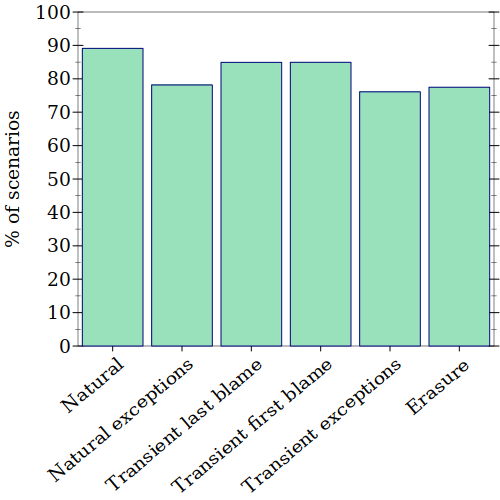
\includegraphics[width=0.40\textwidth]{./plots/success-bars}

  \vspace{1em}
  \begin{minipage}{0.95\textwidth}
  The estimated percentage of scenarios for which each mode succeeds in locating the bug.
  The upper bound margin of error is 0.02\%.
  \end{minipage}

  \caption{Success rates.}
  \label{fig:success-bars}
\end{figure}

\begin{figure}
  \centering
  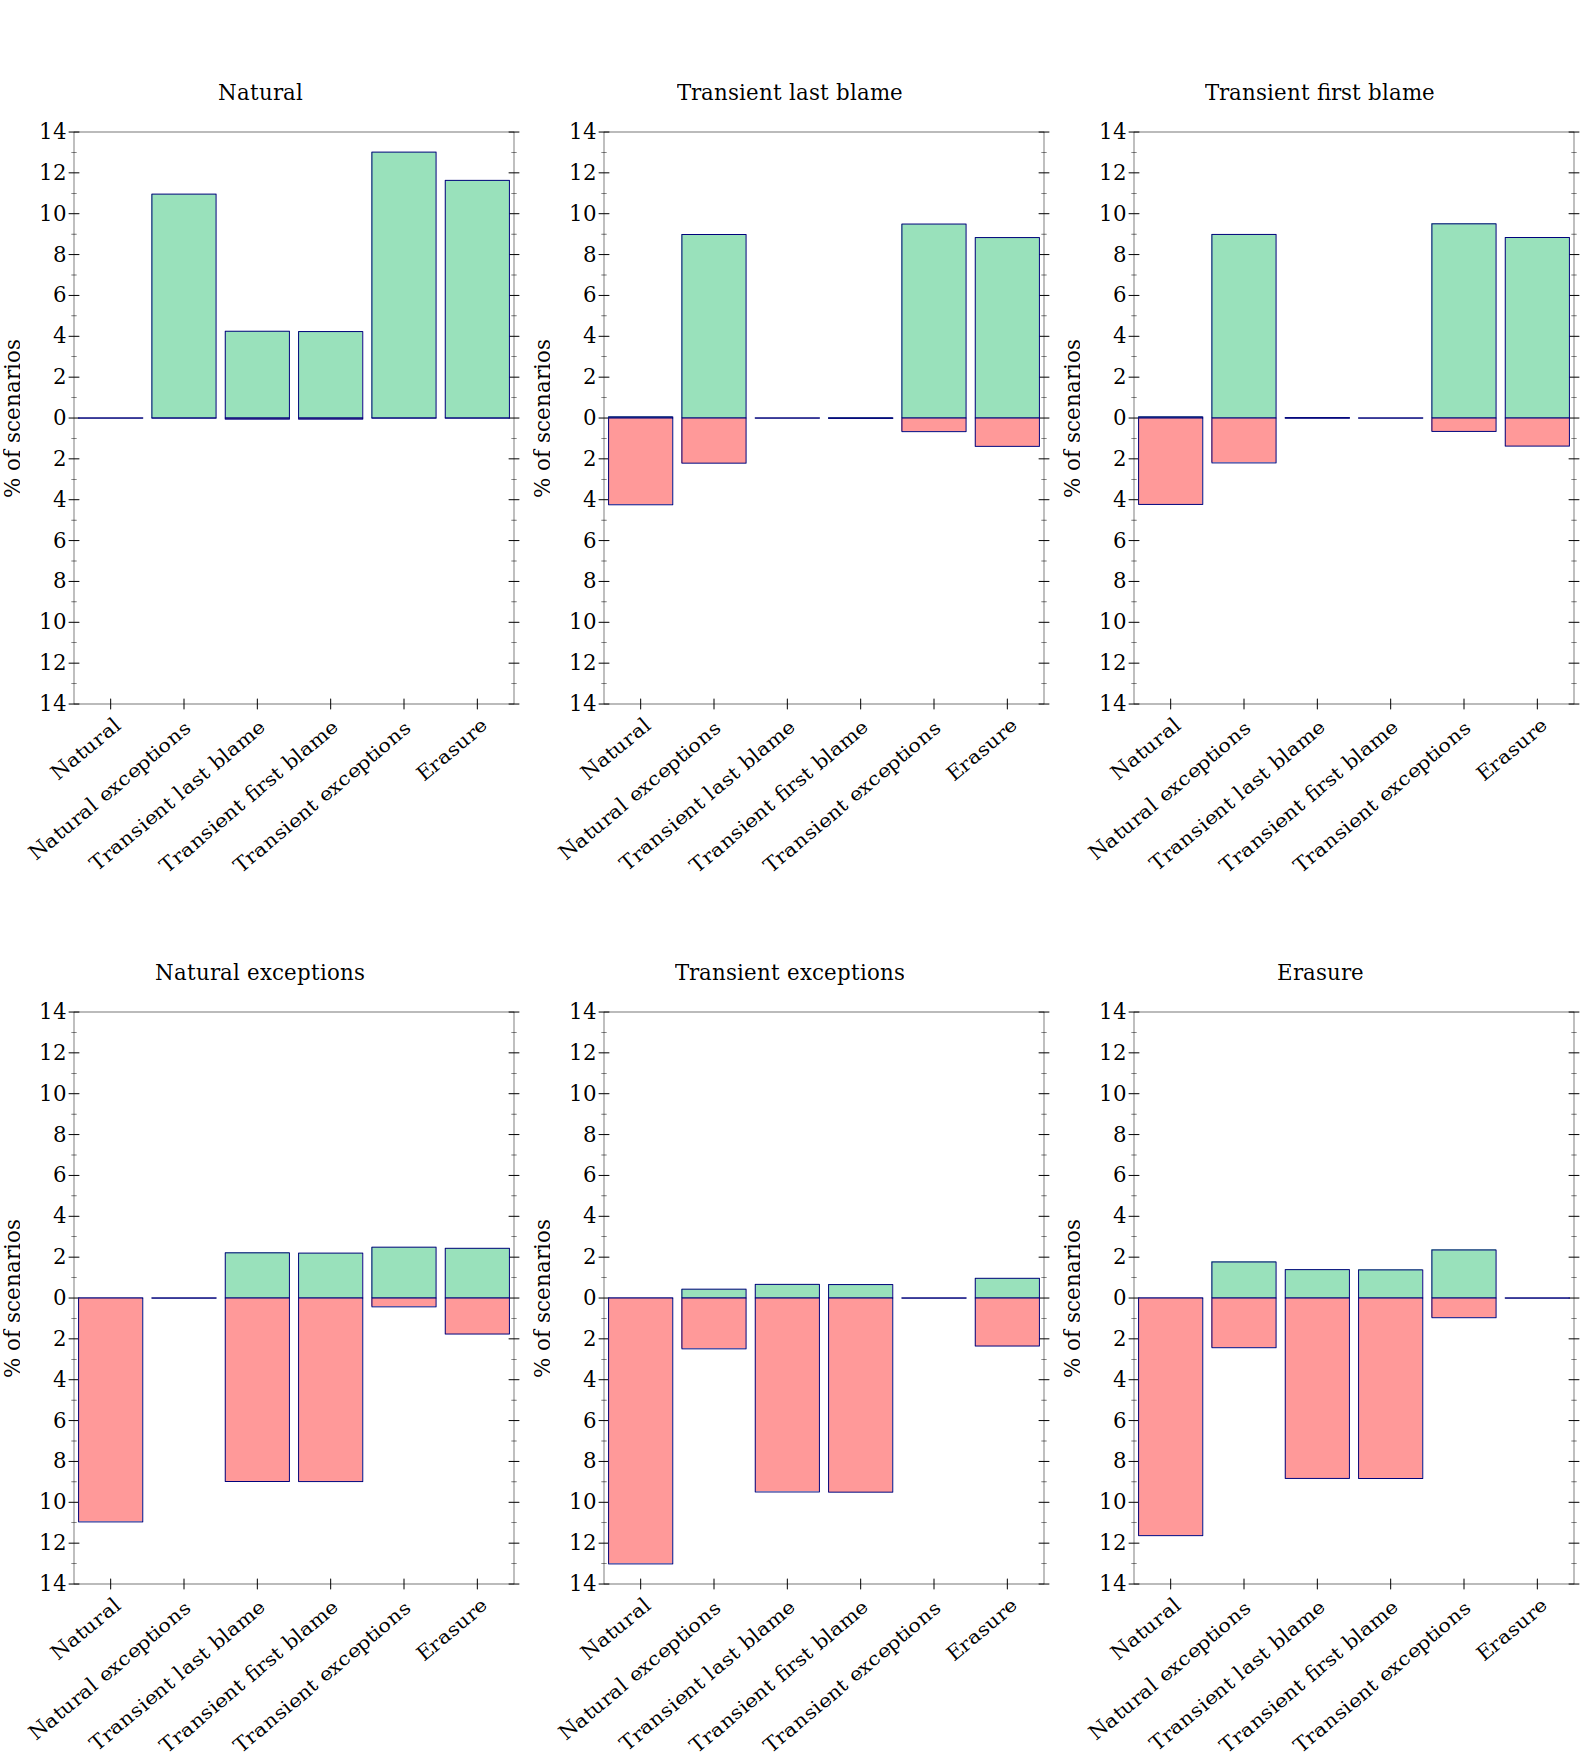
\includegraphics[width=\textwidth]{./plots/avo-bars}

  \vspace{1em}
  \begin{minipage}{0.95\textwidth}
  Each plot depicts a head-to-head comparison of the entitled mode against every other mode.
  The portion above 0 (in green) is the estimated percentage of scenarios where the entitled mode is more useful
    than the other mode.
  The portion below 0 (in red) is the estimated percentage of scenarios
    where the entitled mode is less useful than the other mode.
  The upper bound margin of error is 0.02\%.
  \end{minipage}

  \caption{Usefulness comparisons.}
  \label{fig:avo-bars}
\end{figure}

\begin{figure}
  \centering
  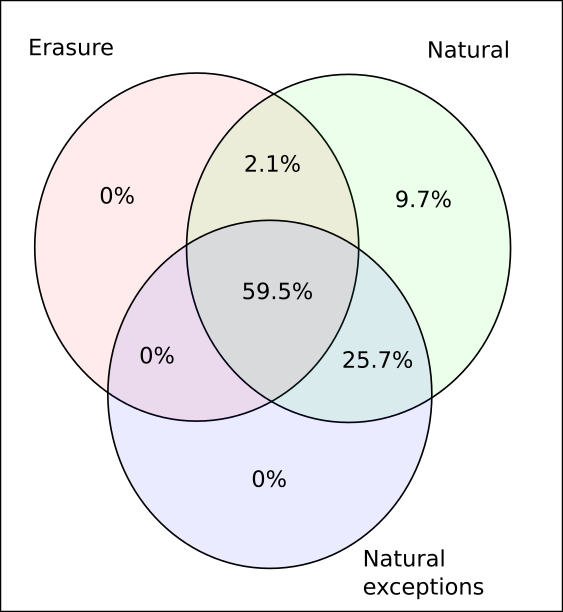
\includegraphics[width=0.32\textwidth]{./plots/TR-TR-stack-first-venn}
  \hfill
  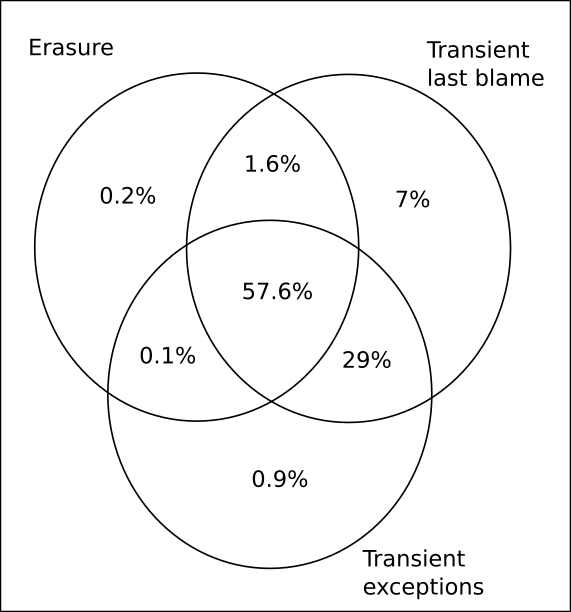
\includegraphics[width=0.32\textwidth]{./plots/transient-newest-transient-stack-first-venn}
  \hfill
  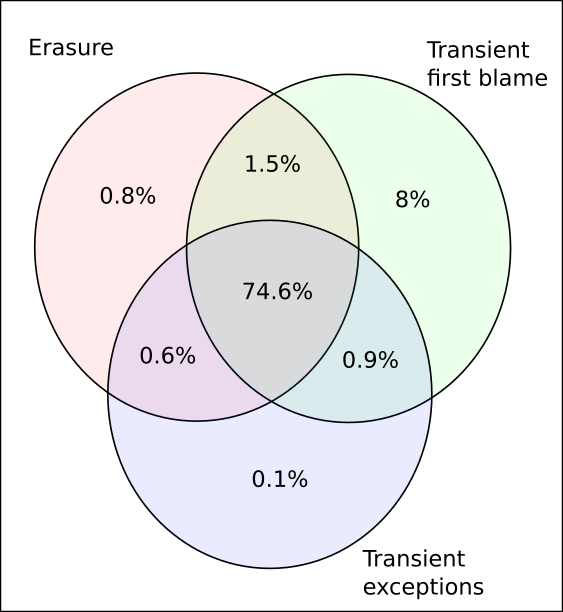
\includegraphics[width=0.32\textwidth]{./plots/transient-oldest-transient-stack-first-venn}

  \vspace{1em}
  \begin{minipage}{0.95\textwidth}
  Each diagram shows the overlap of the successful scenarios for three modes.  
     For example, in the leftmost diagram, all three modes succeed on the
    same scenario 57.3\% of the time, only Natural and Natural exceptions
    succeed on 29.1\% of the scenarios, only Natural and Erasure succeed
    on 2.1\%, and Natural alone succeeds on 9\%.  The upper bound margin
    of error is 0.02\%.
  \end{minipage}

  \caption{Blame usefulness analysis.}
  \label{fig:success-venns}
\end{figure}


Figure~\ref{fig:success-bars} summarizes the overall success rates of
every mode.  The success rates illustrate a few points that underlie the
rest of our analysis.  The first notable piece of information from this
figure is that every mode has failed debugging scenarios, not just
Erasure. This should not come as a surprise to the astute reader.  Running
a mode of the rational programmer on a scenario may result in an exception
that carries no useful information about which module the programmer
should type next. For instance the stack trace of the exception may not
contain frames from any module of the program but only from the internals
of the Typed Racket implementation. This situation can happen at any point
along a blame trail, causing it to fail.

While most failures to debug scenarios follow the above pattern, a few do
not.  Breaking down the reasons for failure for Natural blame (1748 in
total) reveals an additional cause. For a small set of debugging scenarios
(40), Natural produces a run time type error blaming a non-buggy already
typed component. All these cases are due to known open issues with Typed
Racket and class contracts. 

In Transient, similar to Natural, most failures are due to unhelpful
exception information (1851 for both Transient first and last blame).
However, Transient also has a substantial number of failures because
scenarios hit the time and memory limits of our experiment
(\textasciitilde770 scenarios).  Additionally, there are nearly 1,000
cases where Transient reports an empty blame set, leaving the rational
programmer without hints about how to proceed.
Sections~\label{sec:threat:transient} and ~\label{sec:threat:transient2}
explain how both of these causes of failure for Transient affect our
experiment. 

The second key observation from figure~\ref{fig:success-bars} is that the
modes that use blame all outperform those that do not.  In particular,
Natural and both of Transient's blame modes succeed in around 95\% of the
scenarios, while their corresponding exception modes succeed in around
85\% of them and Erasure succeeds in only 60\%.  The only
exception is that the Random programmer always succeeds; this reflects the
fact that every scenario has finitely many modules, so Random programmer 
eventually types the buggy module.


Figure~\ref{fig:avo-bars} depicts a head-to-head comparison of every
mode's performance against every other mode (except Random). The
comparison  answers the four questions from section~\ref{sub:experiment}. 
Each plot shows the proportion of scenarios where one mode performs
better or worse than each other mode.  In particular, each bar above zero
represents the proportion where the plot's entitled mode succeeds and the
mode on the x-axis fails; the corresponding bar below zero represents the
proportion of the inverse case.  For example, the plot titled ``Natural''
shows that Natural outperforms Natural exceptions in about 12\% of the
scenarios, and the inverse (Natural performs worse than Natural
exceptions) never happens.  Similarly, the plot titled ``Transient last
blame'' shows that Transient last blame outperforms Natural exceptions
 in about 12\% of the scenarios, but conversely it performs worse
than Natural exceptions in about 2\% of the scenarios.

The figure answers questions $Q_1$, $Q_2$ and $Q_3$ affirmatively.  
In all three semantics, blame modes outperform their
corresponding exception mode by \textasciitilde10\%.  The
Natural exceptions mode is never more useful than Natural blame, and
Transient exceptions are more useful than Transient first and Transient
last blame in a small percentage (about 2\%) of the scenarios. 

Figure~\ref{fig:avo-bars} also provides answers for $Q_*$.
Blame for all three semantics is significantly
more useful than Erasure exceptions (by around 35\%). Natural blame is
more useful than both versions of Transient blame by a small percentage;
in about 4\% of scenarios Natural blame is more useful while in about 1.5\% of the
scenarios Transient blame is more useful. The Transient first and
Transient last blame are practically indistinguishable. Finally, there is
no clear winner between Natural exceptions and Transient exceptions
despite the theoretically advantageous additional checks of the Natural
semantics.

\begin{figure}
  \centering
  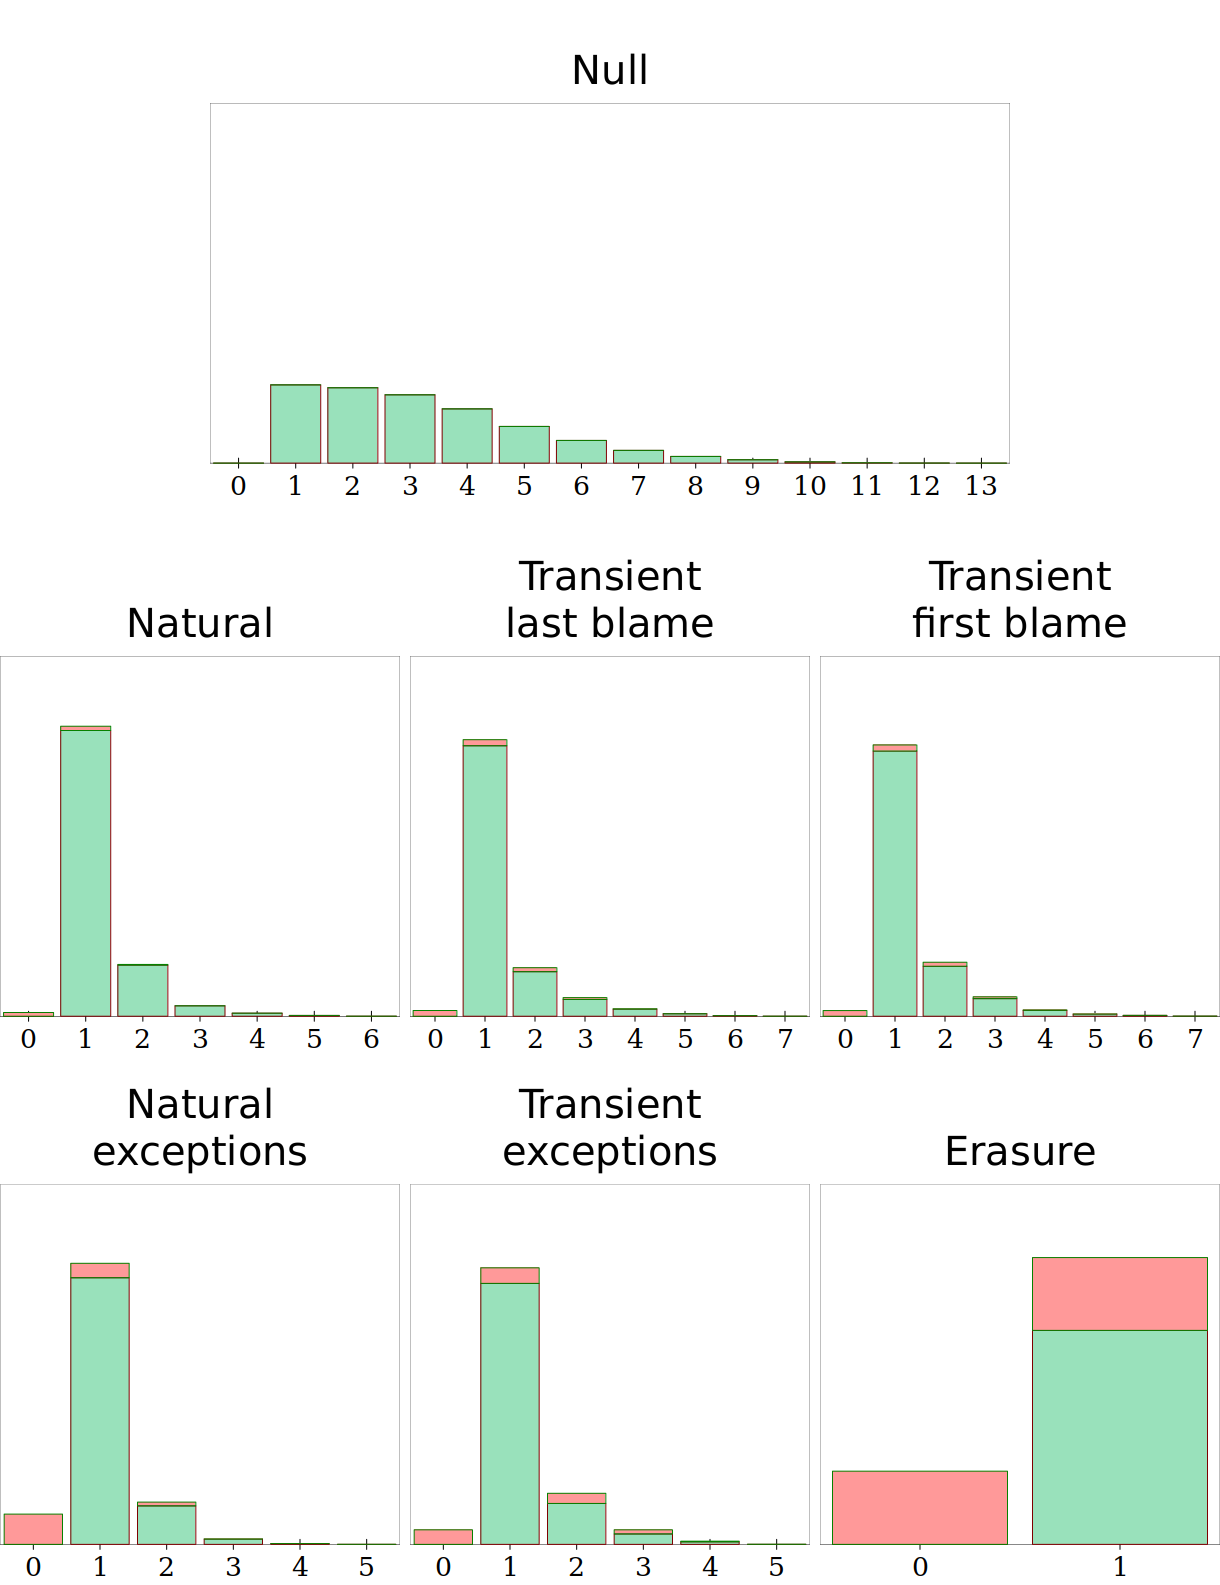
\includegraphics[width=\textwidth]{./plots/bt-lengths-table}

  \vspace{1em}
  \begin{minipage}{0.95\textwidth}
  Each plot depicts the distribution of trail lengths for a given mode across all benchmarks.
  \end{minipage}

  \caption{Programmer effort.}
  \label{fig:effort-table}
\end{figure}

\begin{figure}
  \centering
  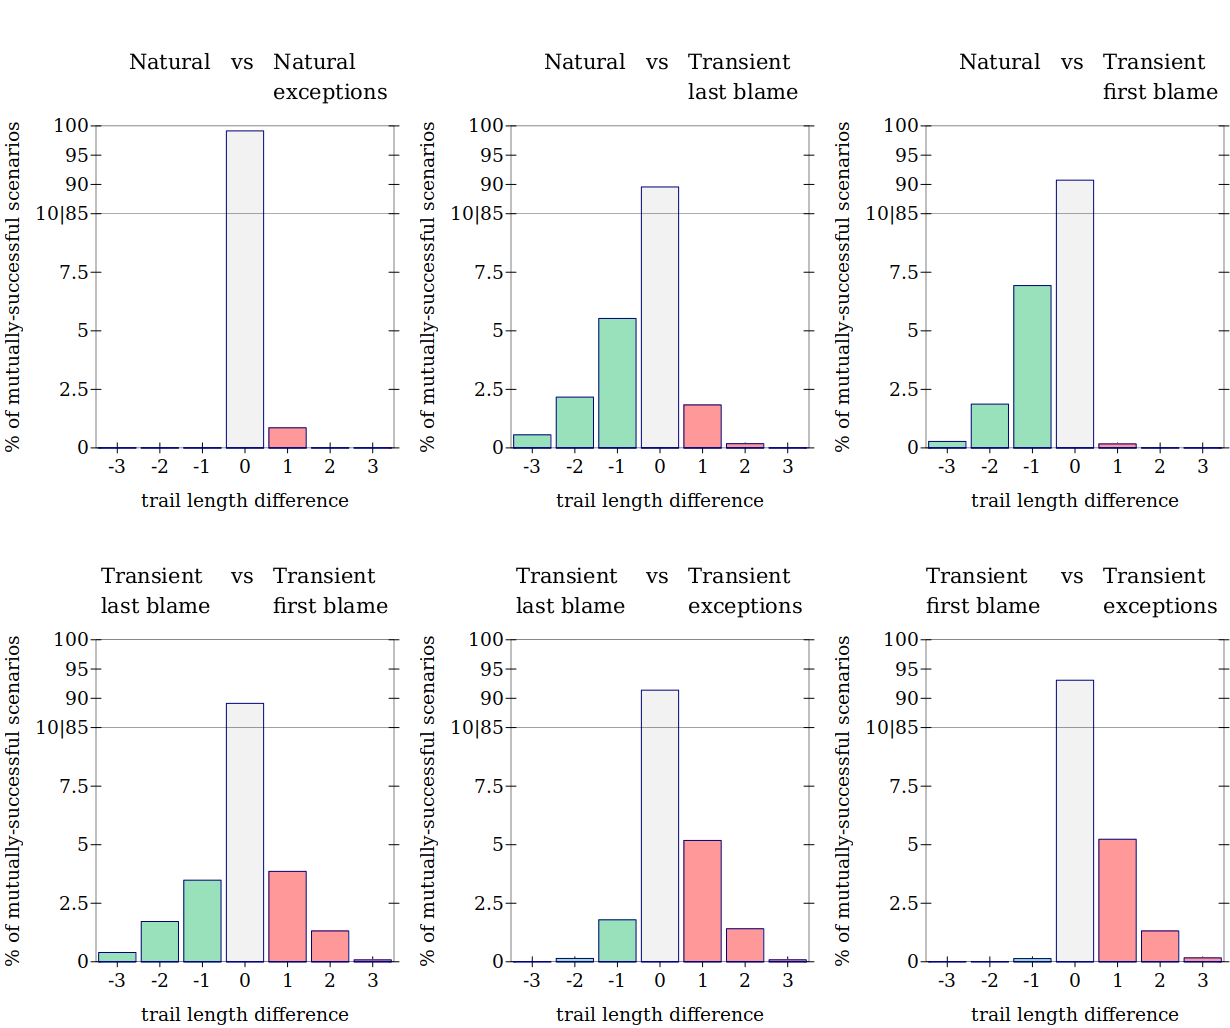
\includegraphics[width=\textwidth]{./plots/bt-length-comparisons}

  \vspace{1em}
  \begin{minipage}{0.95\textwidth}
  Each plot depicts the distribution of scenarios with trail length
    differences ranging from -3 to 3.  A -x difference denotes that
    the first mode's trail is x steps shorter than the second mode's
    trail for the same scenario, and a positive difference denotes the
    inverse.  Only scenarios where both modes succeed are considered.  The
    10|85 on the y-axis indicates that the axis is truncated between 10
    and 85\%.
  \end{minipage}

  \caption{Effort comparisons.}
  \label{fig:effort-comparisons}
\end{figure}

In order to better understand the answers the experiment provides for
questions $Q_1$ to $Q_3$, figure~\ref{fig:success-venns} depicts an
analysis of the success of each semantics in comparison to Erasure.
Specifically, the figure shows one Venn diagram per mode of the rational
programmer that uses blame.  Each diagram shows the overlap of successful
for a  the blame mode, its corresponding exception mode, and Erasure.  For
example, for Natural, the leftmost diagram shows that all three modes
succeed on 59.5\% of the  scenarios, only Natural and Natural exceptions
succeed on 25.7\% of the scenarios, only Natural and Erasure succeed on
2.1\%, and Natural alone succeeds on 9.7\%.  This analysis highlights
the success trade-offs each semantics offers against Erasure, with and
without blame. Hence, it answers questions about how to choose to between
blame or just exceptions for each semantics.  For instance, the analysis
for Natural clearly illustrates that, when choosing between Natural blame,
Natural exceptions, and Erasure, Natural blame is the absolutely most
successful: all of the successes of the other two modes are subsets of
Natural's successful scenarios.  On the other hand, Transient's blame
modes fare similarly but the choice is not so clear-cut.


Turning to programmer effort, figure~\ref{fig:effort-table} shows the
distribution of blame trail lengths for the sampled interesting debugging
scenarios. Unlike the usefulness comparisons above, these proportions do
not generalize to a representation of the full population.  Still, as
section~\ref{subsec:effort} discusses, they provide an alternative view of
the workings of the rational programmer. 

There are two immediate take-aways from the figure. First, the effort for
successfully debugging interesting scenarios (in green) for the random
mode of the rational programmer is highly spread out, as
expected.\footnote{The random mode distribution is indistinguishable for
all three semantics and thus the figure~\ref{fig:effort-table} only shows
one plot.} In contrast, in the other modes, successful effort coalesces at
the left side of the plot, meaning that in most cases the programmer needs
to type a single component to debug a scenario. 

A second point of interest is that the exceptions of the Erasure semantics
either help the rational programmer immediately or the rational programmer
fails to debug a scenario altogether (in red).  This is expected; adding
type annotations to an Erasure program doesn't change it's behavior, so if
the type checker doesn't reject the program with the new annotations, the
rational programmer is stuck.  In other words, an exception from the
runtime has to point to the buggy module with the first try. Otherwise the
rational programmer types an irrelevant module, runs the program again,
and the same exception points again to the already typed module. 

Figure~\ref{fig:effort-comparisons} provides head-to-head comparisons of
effort.  The comparison between two modes boils down to the difference in
length between their trails for all scenarios where they both succeed.
Hence, each plot in the figure shows the distribution of scenarios with
length differences ranging from -3 (the first mode's trail is 3 steps
shorter than the second's) to 3 (the first mode's trail is 3 steps longer
than the second's).  The figure offers several insights about how  modes
compare in terms of effort that complement the insights about how they
compare in terms of success rates from figure~\ref{fig:avo-bars}.  First,
Natural blame never produces shorter trails than Natural exceptions, and
sometimes (albeit rarely) produces slightly longer ones.  Hence, the
experiment provides evidence that blame helps the rational programmer
debug more scenarios but does not shorten the debugging process compared
to exceptions. A second insight is that Natural relatively often (around 10\% of the
scenarios) produces shorter trails than both Transient blame modes, and
sometimes the trails are significantly shorter.  Third, Transient last
blame often produces shorter trails than Transient first blame, which is a
particularly interesting distinction in light of their nearly
indistinguishable success rates.  Finally, Transient's blame modes also
share the characteristic with Natural that blame sometimes produces longer
trails than their corresponding exception modes.

